\documentclass[conference,10pt,letterpaper,final]{IEEEtran}
% \documentclass[10pt,letterpaper, onecolumn]{article} 
\usepackage{times}

\usepackage{graphicx} 
%\usepackage{ifpdf}
% \ifpdf
% \usepackage[pdftex]{graphicx}
% \else
% \usepackage{graphicx}
% \fi
\usepackage{subfigure}
%\usepackage{stfloats}
\usepackage{amsmath}
\usepackage{amssymb}
% \usepackage{amslatex}
\usepackage{amsfonts} 
% \usepackage[ps2pdf=true]{hyperref}
\pagestyle{empty}

%\usepackage{afterpage} 
\hyphenation{Packet-Skip}
\usepackage{multirow,tabularx}
\pdfsuppresswarningpagegroup=1

%\usepackage{flushend}
\usepackage{paralist}

% \hypersetup{% Ä=\304; Ö=\326; Ü=\334
%   ...
\begin{document}

\title{PacketSkip Revisited: Efficient Retrieval of Node Capabilities in Heterogeneous P2P Networks}


\author{Andreas Funke \\
 \textit{Email: andreas.funke@hhu.de}\\
 \textit{University of D\"usseldorf, HHU - 2017 SS - Opportunistic and Peer-to-Peer Networks} \\
 }


\maketitle
\thispagestyle{empty}

\begin{abstract}
In modern miscellaneous peer-to-peer (p2p) networks, combining desktop computers and mobile devices, the homogeneous roles of peers clash with the heterogeneous capabilities of their hosts. Therefore, advanced p2p systems try to allocate heavier load to stronger peers. Identifying and indexing peers by their capacities is an ongoing research. Recently, we have proposed PacketSkip, a Skip Graph based, ordered indexing structure, that provides multidimensional range queries for multi-featured peer capacities. PacketSkip can be added as an additional layer to any DHT-based p2p-overlay. Although its storage demands are already low, storage and update traffic scalability was still of concern for high-dimensional data. Also, the index uses the overlay's lookup mechanism which adds the networks lookup complexity as a factor to its communication's running time.

In this paper, we propose several efficiency optimizations for the PacketSkip protocol which help to reduce storage and traffic costs by avoiding to send and store redundant information. These mechanisms are approximately halving the storage and update traffic costs as evaluation shows. Furthermore, we were able to clearly enhance traffic speed by caching host information of PacketSkip nodes, and thereby avoiding frequent p2p-lookups.
\end{abstract}



\section{Introduction}
\label{sec:introduction}

Peer-to-peer (p2p) systems have become more and more popular in several network applications and services. Due to their self-organizing paradigm, p2p systems avoid a single-point-of-failure and have been proven to be cost-effective, robust and scalable. However, in modern miscellaneous peer-to-peer networks, combining desktop computers and mobile devices, the homogeneous roles of peers clash with the heterogeneous capabilities of their hosts. Weaker hosts that are responsible for important tasks, such as providing popular files, may reduce the overall service quality. Therefore, advanced p2p systems try to allocate heavier load to stronger peers.

Identifying and indexing peers by their capabilities is an ongoing research. Recently, we have proposed PacketSkip, a Skip Graph based, ordered indexing structure, that provides multidimensional range queries for multi-featured peer capacities. Skip Graphs provide a non-hierarchical, distributed data structure where data is arranged in a sorted sequence, access times are logarithmic on average and the graph is robust against node failure. The PacketSkip service inherits and extends these features. PacketSkip can be added as an additional layer to any DHT-based p2p overlay. Although its storage demands are already low, storage and update traffic scalability was still of concern for high-dimensional data. Also, the index uses the overlay's lookup mechanism which adds the networks lookup complexity as a factor to its communication durations.

In this paper, we propose several efficiency optimizations for PacketSkip which help to reduce storage and traffic costs while also boosting performance:

\begin{enumerate}
  \item protocol change: additional features are added to index elements on the receiving node instead of the sending peer
  \item protocol change: additional features are only stored in an index element if they are lexicographically higher
  \item protocol change: a multidimensional search must focus on the feature which is lexicographically lowest
  \item message delivery optimization: adding a node$\rightarrow$host mapping as a communication cache to each node
\end{enumerate}

PacketSkip has been introduced in detail in Funke \cite{packetskip09} and Disterh{\"o}ft et al. \cite{packetskip10}.
%A concise recap follows in Section~\ref{subsec:packetskip}.
From now on we will refer to these previous protocol revisions as (protocol) v0.9 and v1.0, respectively.
The now introduced changes to the protocol, which are discussed in Section~\ref{sec:solution}, will be referred to as v1.1 and v1.2.

The remainder of this paper is organized as follows: first, we briefly discuss related works (Section~\ref{sec:related}). We then give a short introduction to Skip Graphs and recapitulate the protocol versions 0.9 and 1.0 by which PacketSkip was originally defined (Section~\ref{sec:protocol}). Next, we discuss the issues on which we want to elaborate our solutions (Section~\ref{sec:solution}) and present the outcome of our thorough evaluation (Section~\ref{sec:evaluation}). Finally, our conclusion and further suggestions for improvements are discussed in Section~\ref{sec:conclusion}.

\section{Related Work}
\label{sec:related}

For an in-depth overview on Skip Graphs -- the data structure PacketSkip is build on -- we recommend the original papers by Aspnes at al. \cite{Aspnes:2007:SG:1290672.1290674} and Harvey et al. \cite{harvey2003skipnet}. Section~\ref{subsec:skipgraph} contains a short summary.

Other approaches in peer capability retrieval use different data structures.
One branch uses Chord-based~\cite{chord} over-overlays (\cite{adaptivechord}, \cite{Kargar2017147}). 
Another common direction focuses on tree based topologies (SkyEye:~\cite{DBLP:conf/icpads/GraffiKXS08}, CapSearch:~\cite{capsearch}, Dragon:~\cite{carlini2016dragon}). PacketSkip has been evaluated extensively against CapSearch in \cite{packetskip10}.

With SkipCluster~\cite{xu2011new}, there is another recent Skip Graph based approach, but in the form of a hierarchical super-peer structure.
In contrast to the foregoing approaches, PacketSkip is non hierarchical and fully flexible in terms of dimensionality, so that capacity features can be added dynamically without updating protocol or topology. It also provides a complete view of the participating peers and very good accuracy (see \cite{packetskip10}).

\section{PacketSkip Explained}
\label{sec:protocol}

For understanding the optimizations proposed in this paper it is important to understand the protocol of PacketSkip first. In this section we briefly recapitulate the basics of a Skip Graph data structure, followed by a short reminder how PacketSkip elaborates on this design. We complete this summary with a description of the internal representation of data and of the routing protocol that grants access to that data.

PacketSkip is a distributed indexing data structure derived from a Skip Graph. It works as an over-overlay to any DHT-based p2p network and provides a sorted set of index items. The index can be searched via multi-dimensional range queries. The current use case is the retrieval of peer capacities where the capacity features -- such as CPU, storage or bandwidth -- are the dimensions and the peer's contact information is the actual search object. However, PacketSkip is not limited to this use case or to a predefined set of dimensions. It is already possible to index e.g. multimedia data files in PacketSkip and associate their meta data with a certain peer offering them.

The main interface to PacketSkip is a service running on each peer. The service provides access to the index's update and search mechanisms. Also, the service maintains the nodes of the underlying distributed Skip Graph where the data is actually stored. In short: it manages the inter-PacketSkip communication as well as the communication to PacketSkip from the outside. For applications which use the service to store and retrieve index items, the inner workings of PacketSkip are basically a black box. The system itself does not care about the use case of the data. For our purposes we implemented a capacity manager application that stores periodically peer capacities and queries them on demand.

\subsection{Skip Graphs}
\label{subsec:skipgraph}

A Skip Graph is a distributed data structure with logarithmic access times on average. It uses a probabilistic approach to establish edges between its nodes. Nodes in a Skip Graph have no global knowledge and there is no hierarchical differentiation between nodes. The nodes are responsible for a certain range in the feature space and sorted in the graph via this responsibility. The feature space is completely and disjointly divided by the nodes.

Skip graph nodes are linked to other nodes on several doubly linked lists with head and tail of each list also linked -- each one effectively forming a ring. The rings are assigned to different levels. On level 0 all nodes are strung in one global ring. Then recursively: a ring on level $i$, $i \in \{0,\dots,l\}$ and $l$ the currently highest level, is split in two disjoint subsets forming two new rings on level $i+1$. The ordering in the rings is kept intact. The allocation of nodes to rings is done locally when a node joins the graph. While every node is member of the only ring on level 0, for each higher level it choses randomly a sample $s \in \{0, 1\}$ and joins the ring associated to $s$ by connecting with its predecessor and successor (in respect to the ordering). The recursion ends when a node is the only node in a ring on its highest level. In summary: with each new level the number of rings doubles and the distance of the edges between two nodes also doubles (on average) which results in logarithmic access times.

Figure~\ref{fig:skipgraph} shows a schematic Skip Graph with 8 nodes (A,\dots,H) from left to right and the disjoint rings on its three lowest levels (0,\dots,2) from top to bottom.

\begin{figure}[htbp]
	\centering
	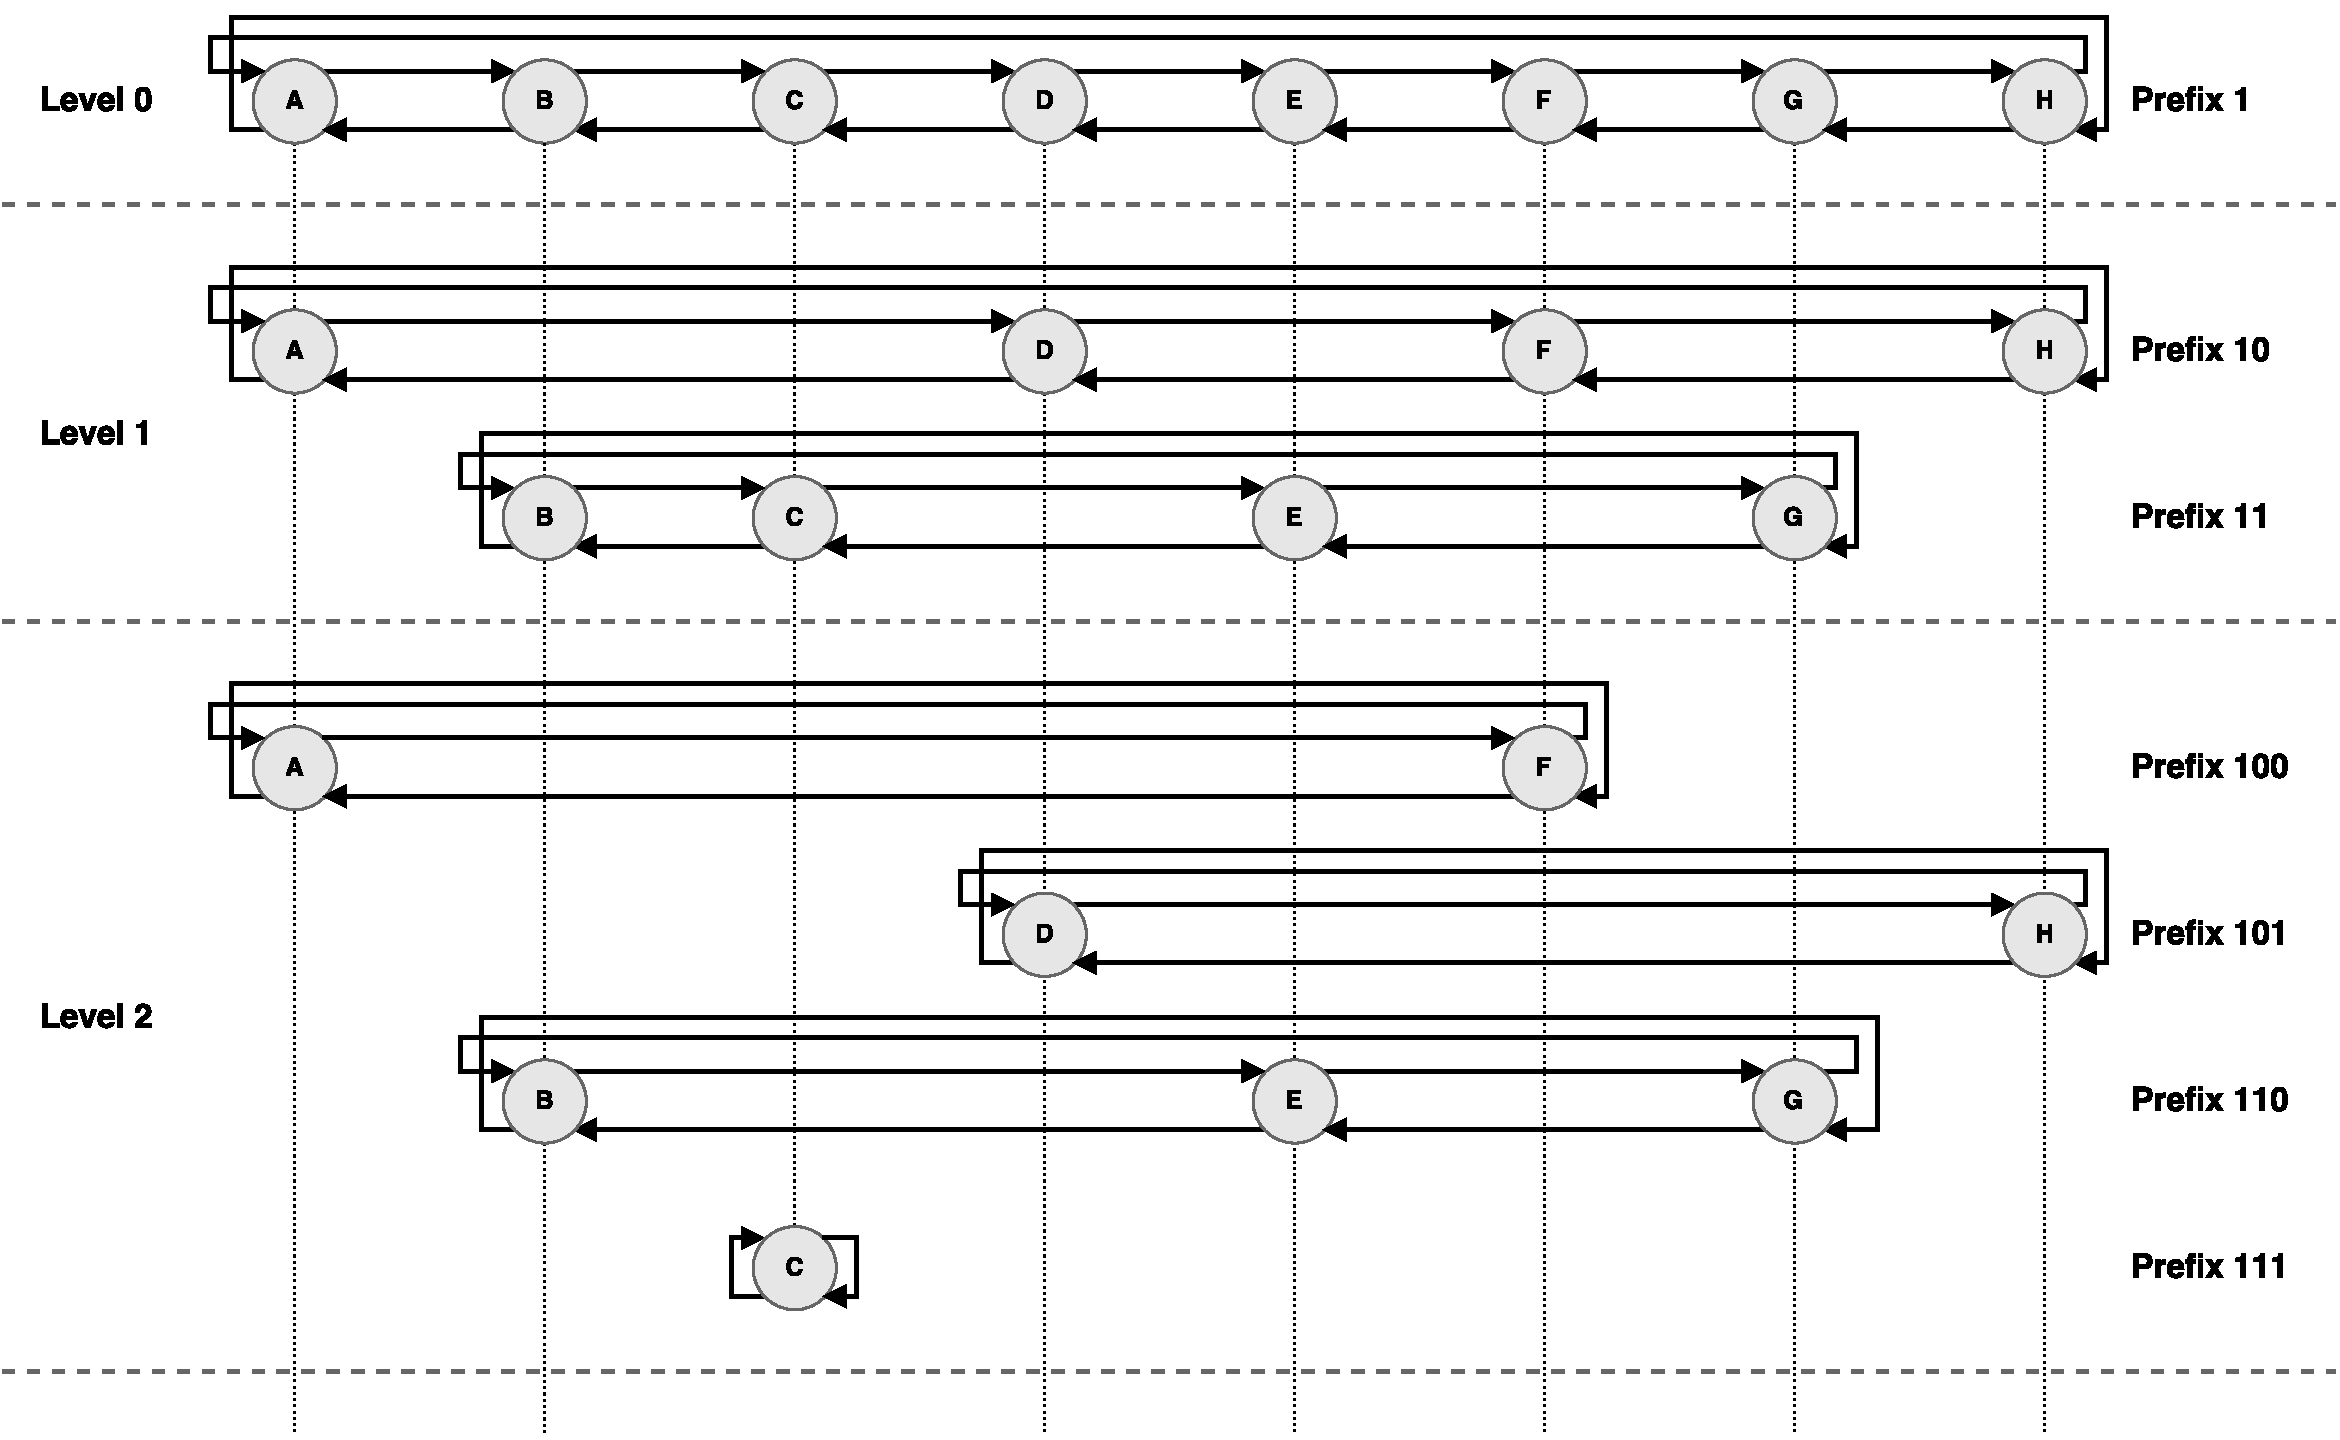
\includegraphics[width=1\linewidth]{graphics/skipgraph}
	\caption{An exemplary Skip Graph}
	\label{fig:skipgraph}
\end{figure}

\subsection{PacketSkip principles}
\label{subsec:packetskip}

The Skip Graph implementation of PacketSkip has little costs in building the graph structure. It is fully reactive and changes the graph structure only regional when nodes join or leave the graph. The join is initiated whenever a node holds too many index items and a leave operation will be performed when a node has too little items. This ensures a good load balancing. The graph will grow linearly with the number of items.

PacketSkip nodes are virtual nodes which reside on a randomly chosen peer. They are DHT objects with a fixed node id out of the overlay's id space. In the default protocol the communication between nodes is fully transparent. Messages to other nodes are addressed to their node ids. Therefore, the underlying overlay has to lookup the peer responsible for a node id with each message delivery. This ensures reliable access in dynamic systems, but it is also costly in terms of time and traffic.

Peers can host a few or no PacketSkip nodes at all. The choice of a random assignment of (PacketSkip) nodes to peers is due to the volatile and random nature of a p2p network under churn. Fixed assignments are almost impossible and load balancing re-assignments would require that node ids must be changed frequently, thereby destabilizing the PacketSkip graph as routing tables had to be updated constantly.

\begin{figure*}[t]
	\centering
	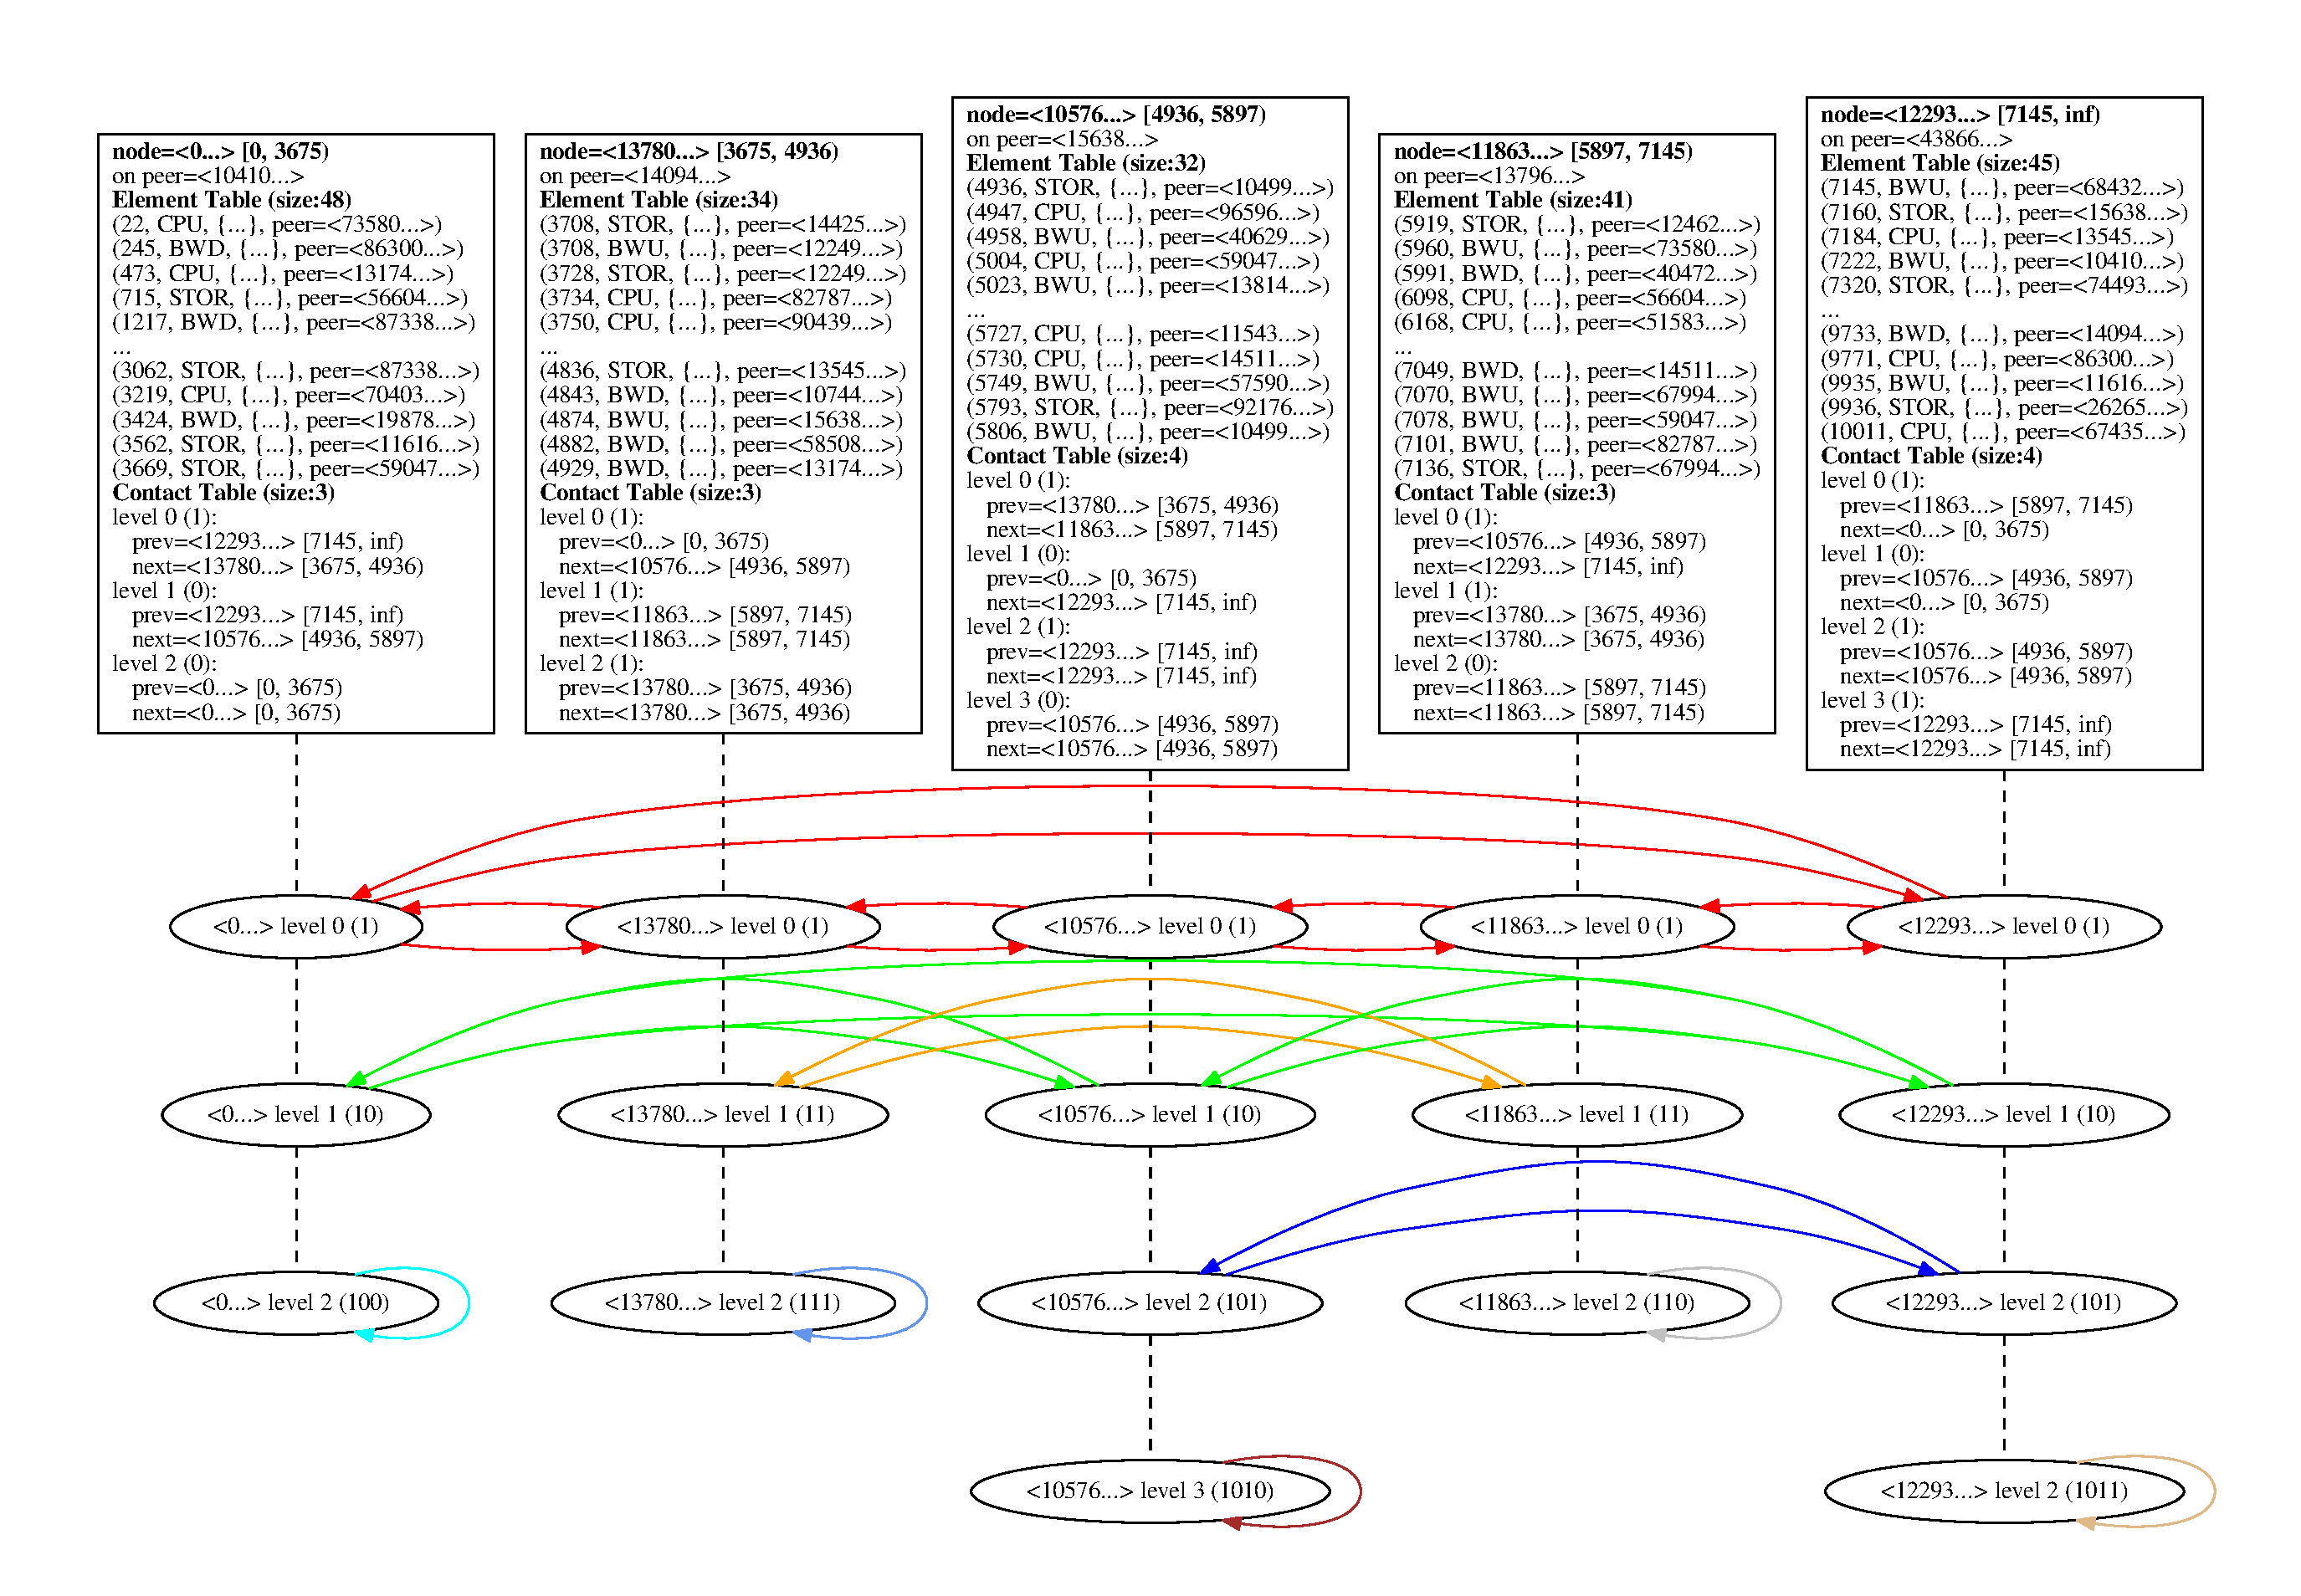
\includegraphics[width=\textwidth]{graphics/packetskipgraph_reduced}%
	\vspace{-0.3cm}
	\caption{An actual small PacketSkip graph. Illustration by Disterh{\"o}ft et al.: PacketSkip~\cite{packetskip10}}
	\label{fig:packetskipgraph}
	\vspace{-0.3cm}
\end{figure*}

Figure~\ref{fig:packetskipgraph} shows an exemplary PacketSkip graph with five nodes. Each node stores index information in an element table and pointers to its neighbors in a routing table. Pointers are visualized as edges in the graph, associated with certain levels in the underlying Skip Graph.

\subsection{Multidimensional data representation}
\label{subsec:datarepresentation}

The full capacity of a peer is described by a set of key-value pair features, for example
$\{CPU\text{:}2400,\;STOR\text{:}9583,\;MEM\text{:}123,\;BW\text{:}5000\}$. 
Whether the values are either precise measures of the given hardware or a mapping to a score is of no concern to PacketSkip as long as the usage is consistent.

In the first design of PacketSkip (v0.9) these features were plainly transformed to index items, which we call PacketSkip elements. These elements are tuples in the form: 
$(\langle key\text{=}feature\text{-}value\rangle,\;\langle feature\text{-}id\rangle,\;\langle peer | host\text{-}id\rangle)$. 
The example above results in four elements:
\begin{equation*}
\begin{split}
(2400,\;CPU, \;peer\text{=}x | ip(x)\text{:}port(x)) \\
(9583,\;STOR,\;peer\text{=}x | ip(x)\text{:}port(x)) \\
(123, \;MEM, \;peer\text{=}x | ip(x)\text{:}port(x)) \\
(5000,\;BW,  \;peer\text{=}x | ip(x)\text{:}port(x))
\end{split}
\end{equation*}

\subsection{Update and search protocol}
\label{subsec:updateandsearch}

A peer announces its capacity information to a random PacketSkip node. The node will then greedily forward the elements to its contacts according to their responsibility ranges, i.e. sending each element to the contact whose responsibility range is closest to the elements key. An element will eventually be stored in the element table of the responsible node. Feature ids are irrelevant for the distribution of elements. All features share the same one-dimensional feature space. Feature id and peer id guarantee the uniqueness of elements.

Each element is tagged with a timestamp. To avoid keeping non-active members, especially under churn, elements will be pruned after a certain time. Therefore, peers must update their capacity information on a regular basis. They may also propagate deletions of obsolete values when a capacity feature has changed, to increase search accuracy. Deletions are distributed exactly as insertions of updated values.

To establish a multidimensional search peers can formulate individual range queries for a set of capacity features. 
A search can be formulated like 
$\{CPU\text{:}[999,2730],\;STOR\text{:}[5000,6000],\;BW\text{:}[5000,\infty)\}$.
These queries are sent to a random PacketSkip node. In the original design the node will split each range queries according to the responsibilities of its contacts and forward them just as updates via a divide and conquer approach. While PacketSkip elements are one-dimensional points in the feature space, search queries are one-dimensional ranges in the same features space. So, distributing range queries inside PacketSkip used to be costly in v0.9 since many nodes could be involved. Also, as PacketSkip elements were one-dimensional, the multidimensionality of a query would not be taken into account inside PacketSkip. Each range used to be regarded individually. This led to many one-dimensional search result messages sent to the seeker which finally had to build an intersection of all these results.

While this first protocol kept update traffic and storage costs to a minimum, the search behavior was indifferent to the multidimensional data, caused too much traffic and did not scale well in terms of search traffic costs. In a revised version of the protocol (v1.0) we vastly improved the search behavior with some trade-off to update and storage costs. A peer adds now additional information to each PacketSkip element in the form of a set of all other features. The element tuples have been extended to the form 
$(\langle key\text{=}value\rangle,\;\langle feature\text{-}id\rangle,\;\{\langle additional\text{ }features\rangle \},$ $\langle peer | host\text{-}id\rangle )$.
For example:
\begin{equation*}
\begin{split}
(2400,\;CPU,  \;\{STOR\text{:}9583,  \;MEM \text{:}123,  \;BW\text {:}5000\}, \\ peer\text{=}x | ip(x)\text{:}port(x)) \\
(9583,\;STOR, \;\{CPU \text{:}2400,  \;MEM \text{:}123,  \;BW\text {:}5000\}, \\ peer\text{=}x | ip(x)\text{:}port(x)) \\
(123, \;MEM,  \;\{CPU \text{:}2400,  \;STOR\text{:}9583, \;BW\text {:}5000\}, \\ peer\text{=}x | ip(x)\text{:}port(x)) \\
(5000,\;BW,   \;\{CPU \text{:}2400,  \;STOR\text{:}9583, \;MEM\text{:}123 \}, \\ peer\text{=}x | ip(x)\text{:}port(x))
\end{split}
\end{equation*}

With such additional information at hand, a multidimensional search does not need to search for each dimension individually, but can focus on one dimension. It adds only elements to the result set which also meet the search criteria for their additional features. The dimension to perform the search on is chosen via the shortest range of all dimensions. 
Our exemplified search is reformulated to
$\{STOR\text{:}[5000,6000],\; \{CPU\text{:}[999,2730],\; BW\text{:}[5000,\infty)\}\}$, where $STOR$ has been chosen as the primary search range and $CPU$, $BW$ are evaluated on the additional feature sets.

Since the intersection of all dimensions is now directly evaluated on the responsible node, the system becomes capable of taking the number of search results into account. A search can therefore terminate after a given number of $k$ results. Actually, since the search is run in parallel on various nodes within the search interval, the number of returned results is mostly greater than $k$, but still clearly smaller compared to a full search.

\subsection{Discussion}
\label{subsec:discussion}

Admittedly, with such improvements to the search behavior in v1.0, there comes an issue to the scalability of update and storage costs. While the search traffic scales very well now, the addition of all features to each index element is of some concern. In this paper we propose a simple mechanism to almost halving these costs by storing only lexicographical suffixes of index items as additional features. There is a small but tenable impact to the search.

Another topic that left room for improvement, is the search and update behavior in regard to its time complexity. As a Skip Graph has $O(\log{m})$ access on average, so has PacketSkip's update and search protocol -- from the viewpoint of the graph with $m$ being the number of PacketSkip nodes. But messages are delivered to node ids which are assigned to responsible peers. A concerned peer must be looked up first. In common structured p2p systems this has $O(\log{n})$ complexity where $n$ denotes the number of peers in the overlay. So, from the viewpoint of the overlay, PacketSkip's has actually an average access time of $O(\log{n} \cdot \log{m})$\footnote{With all other parameters fixed, $m$ is in linear relation to $n$, therefore we can approximate with $O(\log^2{n})$.}
-- regardless of the protocol. We have addressed this issue by caching foreign host information on PacketSkip nodes and achieved roughly true $O(\log{m})$ running time, as explained in Section~\ref{subsec:cache}.

\section{PacketSkip Improvements}
\label{sec:solution}

In this section, we first describe our solution for the storage and update message issue. Secondly, we present our approach for a host cache.

\subsection{Protocol revisions}
\label{subsec:revisions}

Version 1.0 of the PacketSkip protocol had a notable redundancy in the content of update messages sent to PacketSkip. 
The additional features were added to the index elements on the sending peer. Additional features are basically a copy of all other elements in the update set. As long as all features are sent in one message, as is the case when sending an update to an entry node of PacketSkip, the additional feature sets per element contain no essential information. The additional feature sets become only relevant when index items are dispersed on several nodes. Therefore, it is sufficient when the receiving entry node of PacketSkip builds the additional feature sets from all other index elements. This is the first change in the protocol (v1.1). Via this simple change we avoid adding capacity information multiple times to one update message. Since update messages to PacketSkip are frequent and sent by all peers in the overlay, this has a noticeable effect on the overall maintenance traffic costs.

In addition, v1.2 reduces redundancy on the storage side and on PacketSkip's inner update traffic. The goal was to not impact the general positive behavior introduced in v1.0. Some concessions to the search duration were nevertheless necessary. If search duration is paramount, v1.2 can be regarded as an option. Before adding additional features to an index element, all features are sorted lexicographically by their feature id. We regard all features as items in an ordered transaction set. In our example the ordered transaction would be $\{ BW,\;CPU,\;MEM,\;STOR \}$. Then we will add only those features to the additional feature set of an index element which are suffixes of is feature id in regard to its ordered transaction set. In our example this will lead to the following elements:
\begin{equation*}
\begin{split}
(5000, \;BW,   \;\{ CPU\text{:}2400, MEM\text{:}123, STOR\text{:}9583 \}, \\ \;peer\text{=}x | ip(x)\text{:}port(x)) \\
(2400, \;CPU,  \;\{ MEM\text{:}123, STOR\text{:}9583 \},                  \\ \;peer\text{=}x | ip(x)\text{:}port(x)) \\
(123,  \;MEM,  \;\{ STOR\text{:}9583 \},                                     \;peer\text{=}x | ip(x)\text{:}port(x)) \\
(9583, \;STOR, \;\{ \},                                                      \;peer\text{=}x | ip(x)\text{:}port(x))
\end{split}
\end{equation*}

We have now reduced the costs for additional features from $(d-1)^2$ to $(d^2-d)/2$ with $d$ being the number of all features. Our costs may still be in $O((d-1)^2)$, but the practical effect is a reduction of 50\% of the storage and update costs for the additional features introduced in v1.0.

In v1.0 a peer was allowed to choose the feature with the smallest search range as a primary feature. With revision v1.2 we must omit this free choice. Instead, the main feature is now determined by the lexicographical order. An entry node will sort the search dimensions lexicographically and search for the feature with the smallest id. For example: $\{ BW\text{:}[5000,\infty), \;\{ STOR\text{:}[5000,6000], \;CPU\text{:}[999,2730] \} \}$. This will guarantee that all features, which are lexicographically higher than the main feature, are included in any index element. The search protocol of v1.0 can remain identical as to the rest. Secondary features are still taken into account on each potential search result, before sending a result set to the seeker.

The following is noteworthy: performing a search on the dimension with the shortest range will not necessarily lead to a minimum amount of search hops or to the shortest search duration. First of all, there is a random factor by choosing an arbitrary entry node, which is unavoidable for good load balancing. Such an entry node may be further away from the shortest range than from a longer range. More importantly, the number of nodes responsible for a given range depends heavily on the distribution of the index elements. Given a normal distribution, a short range close to the mean may result in more search hops than a broad range close to the tail of the distribution. So, the drawback of not choosing the shortest range is somewhat alleviated.

\subsection{Communication host cache}
\label{subsec:cache}

We introduced a cache to PacketSkip nodes that maps node ids to actual hosts. Each node has its own cache. The cache is not part of the DHT object, but maintained by the PacketSkip service running on a peer. When a node switches to a different peer under churn, the cache is therefore reset. Incoming messages already contain information of the sending host (ip, port), the sending peer (peer id) and the sending node (node id). With each incoming message the cache mapping is updated, with the node id being the key and the host information being its value. Before sending a message to another node, the sender looks up the host information for a given node id from the cache and sends the message directly to this host. A lookup via the p2p overlay is thus bypassed. 

There can be cache misses when a peer either leaves the overlay or the responsibility for a PacketSkip node has changed. In this case, a traditional overlay lookup is performed and the node$\rightarrow$host mapping will be removed from the cache. A cache miss is identified when the sender hasn't received an ACK up to a certain timeout. Since we assume that a direct message to an online host should result in a fast ACK we can set the timeout quite strictly. This will avoid a notable latency for cache misses. Choosing the timeout too strictly can lead to redundant messages. The choice for an appropriate timeout may be host dependent and can also be included as additional information in the host cache.

% This is however beyond the scope of this paper since we have evaluated with a constant net latency.

\section{Evaluation}
\label{sec:evaluation}

\begin{table}[t]
  \caption{Simulation Parameters}
  \label{tab:eval_param}
  \centering
  \begin{tabular}{|c|c|}
  \hline
  \textbf{Parameter}       & \textbf{Values} \\
  \hline
  \hline
  Simulation time          & 330 minutes \\
  \hline
  Number of seeds          & 10 \\
  \hline
  Capacity change interval & all 30 minutes \\
  \hline
  Capacity dimensions      & 3 (scenarios A,B), 5 (scenario C) \\
  \hline
  Search interval          & 2 searches per minute in total \\
  \hline
  Number of nodes (seekers) & 1000 (240) \\
  \hline
  Full-/k-search           & k=8, full \\
  \hline
  P2P overlay              & Chord \\
  \hline
  Element table size       & 50 \\
  \hline
  Network dynamics         & Smooth capacity change \\
  \hline
  Overlay churn            & Inactive (A), Active from min. 161 (B,C)\\
  \hline
  Network layer model      & Simple \\
  \hline
  Cache timeout            & 50ms \\
  \hline
  \end{tabular}
\end{table}

\begin{table}[t]
  \caption{Simulation Scenario}
  \label{tab:eval_scenario}
  \centering
  \begin{tabular}{|r|l|}
  \hline
  \textbf{Period of time (in minutes)} & \textbf{Action performed} \\
  \hline
  \hline
  0 -- 90 & Overlay join\\
  \hline
  91 -- 120 & Do nothing (stabilize overlay) \\
  \hline
  121 -- 130 & Start the PacketSkip service \\
  \hline
  131 -- 190 & Start periodic capacity changes \\
  \hline
      200 -- 320 & Perform full- or k-searches \\
  \hline
      330 & End of simulation \\
  \hline
  \end{tabular}
\end{table}




\begin{figure}[htbp]
  \centering

  \subfigure[A: 1.0 $\rightarrow$ 1.1 $\rightarrow$ 1.2 -- Outgoing traffic, 3 features, no churn\label{fig:traffic_peers_A_out}] {\centering
  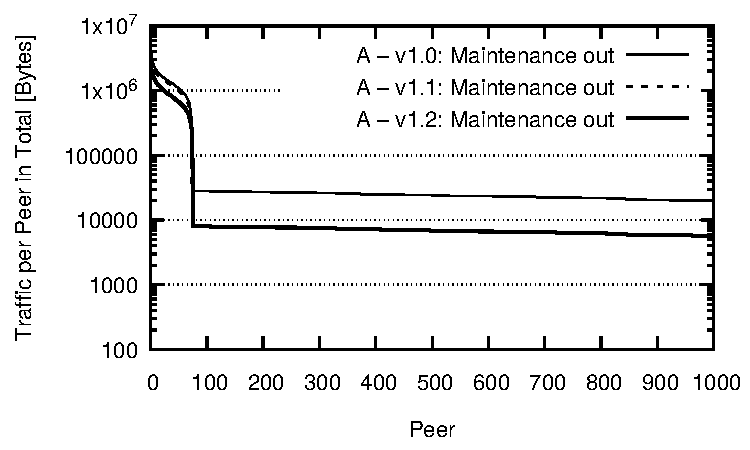
\includegraphics[width=0.98\linewidth]{graphics/fig/Maintenance_Traffic_Peers_A_out}
  }
  \\[-1ex]
  \subfigure[A: 1.0 $\rightarrow$ 1.1 $\rightarrow$ 1.2 -- Incoming traffic, 3 features, no churn\label{fig:traffic_peers_A_in}] {\centering
  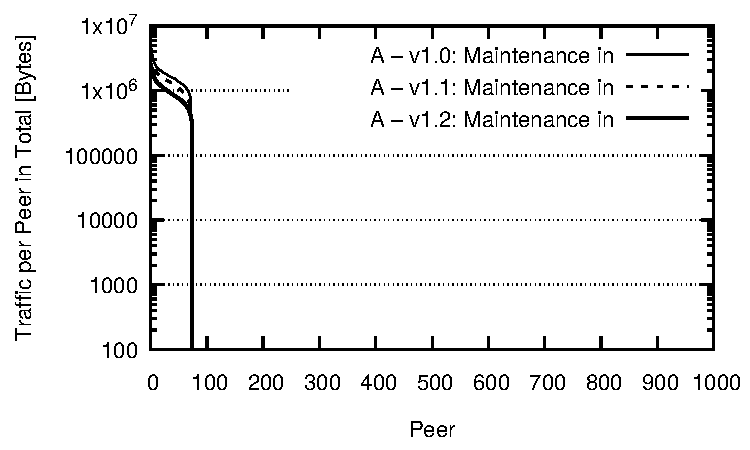
\includegraphics[width=0.98\linewidth]{graphics/fig/Maintenance_Traffic_Peers_A_in}
  }
  \\[-1ex]
  \subfigure[C: 1.0 $\rightarrow$ 1.1 $\rightarrow$ 1.2 -- Outgoing traffic, 5 features, churn\label{fig:traffic_peers_C_out}] {\centering
  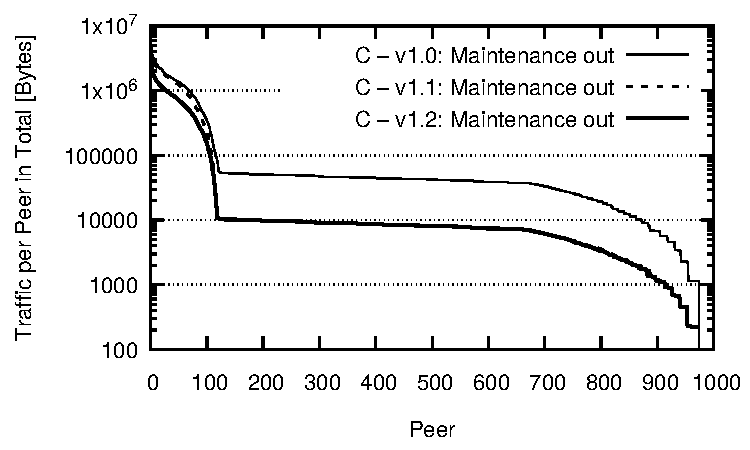
\includegraphics[width=0.98\linewidth]{graphics/fig/Maintenance_Traffic_Peers_C_out}
  }
  \\[-1ex]
  \subfigure[C: 1.0 $\rightarrow$ 1.1 $\rightarrow$ 1.2 -- Incoming traffic, 5 features, churn\label{fig:traffic_peers_C_in}] {\centering
  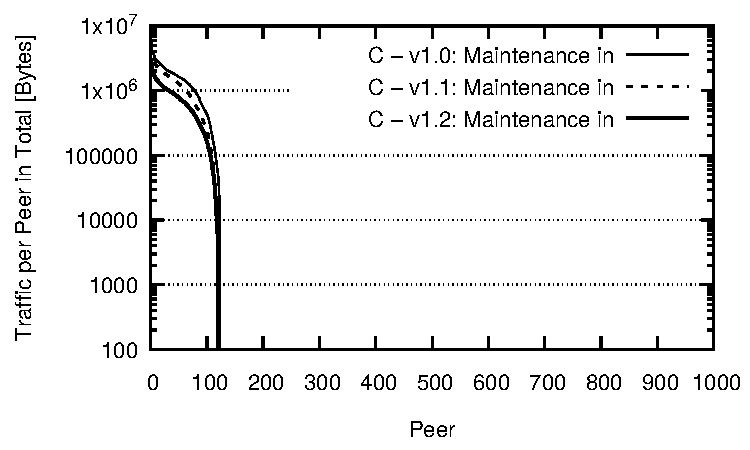
\includegraphics[width=0.98\linewidth]{graphics/fig/Maintenance_Traffic_Peers_C_in}
  }
  \\[-1ex]

  \caption{Protocol revisions v1.1 + v1.2 -- maintenance traffic by peers}
  \label{fig:traffic_peers}
\end{figure}

\begin{figure}[htbp]
  \centering

  \subfigure[A: 1.0 $\rightarrow$ 1.1 $\rightarrow$ 1.2 -- 3 features, no churn\label{fig:traffic_time_A}] {\centering
  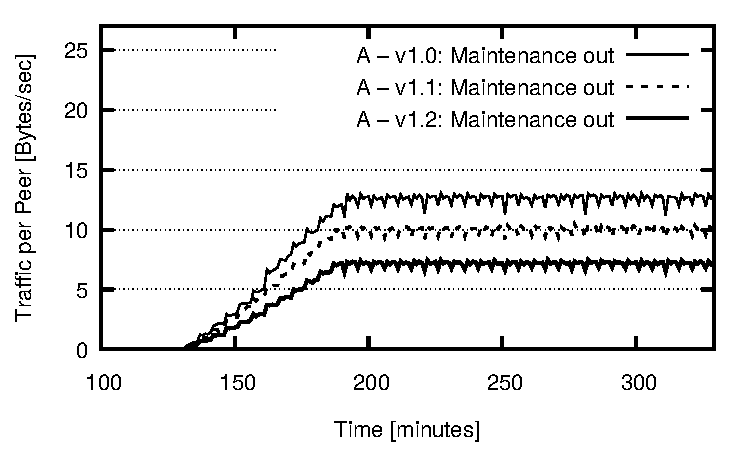
\includegraphics[width=0.98\linewidth]{graphics/fig/Maintenance_Traffic_Time_A_11+12}
  }
  \\[-1ex]
  \subfigure[C: 1.0 $\rightarrow$ 1.1 $\rightarrow$ 1.2 -- 5 features, churn\label{fig:traffic_time_C}] {\centering
  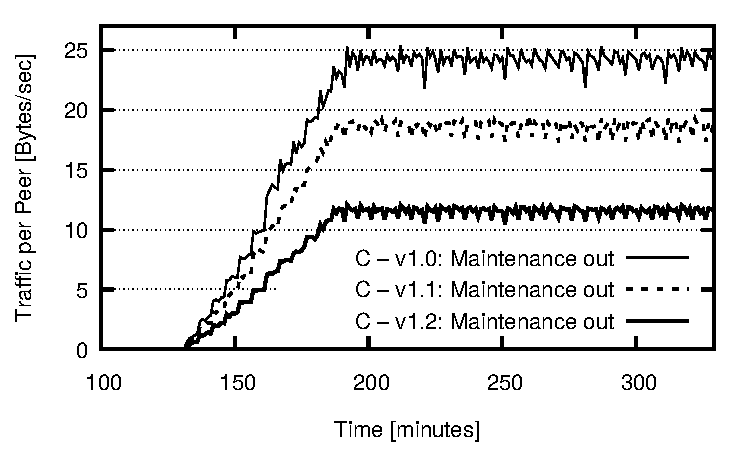
\includegraphics[width=0.98\linewidth]{graphics/fig/Maintenance_Traffic_Time_C_11+12}
  }
  \\[-1ex]

  \caption{Protocol revisions v1.1 + v1.2 -- maintenance traffic by time}
  \label{fig:traffic_time}
\end{figure}


For evaluating the protocol revisions our metrics are 
\begin{inparaenum}[i)]
  \item maintenance traffic costs to PacketSkip,
  \item maintenance traffic costs between PacketSkip nodes,
  \item storage costs,
  \item impact on search duration and search hops and
  \item global PacketSkip traffic costs.
\end{inparaenum}
For the evaluation of the host cache we examine the following metrics:
\begin{inparaenum}[i)]
  \item search and update duration,
  \item performance under churn and
  \item effects on global overlay traffic costs.
\end{inparaenum}

PacketSkip has been implemented in the PeerfactSim.KOM~\cite{peerfactsim} p2p simulator. All changes are evaluated inside this simulation framework. For consistency we rely on the basic scenarios already introduced in \cite{packetskip10}. See Table~\ref{tab:eval_scenario} for details. Scenario A runs without churn, while scenario B and C uses churn with a Kad-distribution. Scenarios A and B use 3 capacity features, with scenario C we used 5 features. For each basic scenario a $k=8$ search and a full search have performed.

For comparison of the different revisions each basic scenario has been simulated with the following parameters:

\begin{enumerate}
  \item[1.0)] protocol v1.0 (as reference)
  \item[1.0c)] protocol v1.0 + cache
  \item[1.1)] protocol v1.1 (adding additional features on the receiving node, not using the suffix model)
  \item[1.2)] full protocol v1.2 (restrict additional features to lexicographical suffixes, includes v1.1)
  \item[1.2c)] full protocol v1.2 (includes v1.1) + cache
\end{enumerate}

We will not expand on all possible combinations A:1.0 to C:1.2c, but only on those with meaningful relevance. Scenario C for example is mostly of interest for the protocol changes and not for the host cache. All scenarios have been simulated with 10 different seeds. For a full overview on all parameters, please refer to Table~\ref{tab:eval_param}. We have used an ideal net layer with a small, constant latency and also a fixed timeout for cache misses.







\subsection{Protocol revision v1.1 and v1.2 -- maintenance traffic costs}
\label{subsec:11}

At first, we evaluate the effects of the protocol enhancement on messages sent to and between PacketSkip nodes.
Figure~\ref{fig:traffic_peers} illustrates the incoming and outgoing maintenance traffic of the service, which includes messages for graph maintenance and especially for index updates, sorted by peers (highest load to the left). The bump on the left side is caused by peers which maintain a PacketSkip node. Peers on the right side are just pushing their update messages. 
For the latter the reduction in output message traffic from v1.0 to v1.1 is apparent.
This was to be expected, since v1.1 eliminates redundancies in update messages sent to PacketSkip.
As v1.2 incorporates v1.1, the effects are identical here (Fig.~\ref{fig:traffic_peers_A_out}: curves of v1.1 and v1.2 are overlapping).
Peers with PacketSkip nodes see positive effects on the incoming side (Fig.~\ref{fig:traffic_peers_A_in}). 

V1.2 on the other hand also reduces the traffic costs inside PacketSkip, demonstrated by less deflection on the left side. This is due to the reduced sizes of the additional feature sets. The effects become more obvious with an increased number of features (scenario C, Fig.~\ref{fig:traffic_peers_C_out}, \ref{fig:traffic_peers_C_in}).
% With 5 capacity features, the number of PacketSkip nodes increases, broadening the bump on the left to some extent. The drop-off to the right is simply caused by churn.

If we average the maintenance traffic over all peers, we notice the effects on the overall maintenance costs of PacketSkip, i.e. messages to the service and between the nodes. There is a noticeable reduction from v1.0 (12.6 Bytes/sec) to v1.1 (10.0 Bytes/sec) to v1.2 (7.2 Bytes/sec) (3 features -- Fig.~\ref{fig:traffic_time_A}), respectively from 24.2 to 18.6 to 11.5 Bytes/sec (5 features -- Fig.~\ref{fig:traffic_time_C})








\subsection{Protocol revision v1.2 -- storage costs}
\label{subsec:dht}

The second protocol revision stores only lexicographical suffixes as additional features. Evaluation proofs that halving the additional features leads to a significant drop of storage requirements, especially with increasing dimensionality (see Fig.~\ref{fig:dht} -- note the log scale of the abscissa). The steps represent peers with one or more PacketSkip nodes. Storage requirements grow almost linearly with the number of nodes a peer maintains. Averaging on all peers, we have measured a reduction from 0.38 to 0.23 KBytes (3 features) and 0.60 to 0.33 KBytes (5 features), which is consistent with the prediction.

  \begin{figure}[htbp]
    \centering
    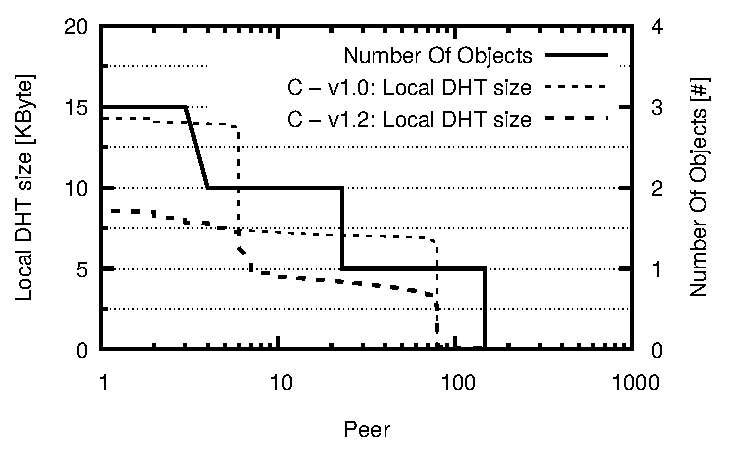
\includegraphics[width=0.98\linewidth]{graphics/fig/DHTSize_PeersSort_C}
    \\[-1ex]
    \caption{C: 1.0 $\rightarrow$ 1.2 -- Storage requirements per peer, 5 capacity features}
    \label{fig:dht}
  \end{figure}



\subsection{Protocol revision v1.2 -- search performance}
\label{subsec:search}

\begin{figure}[htbp]
  \centering

  \subfigure[A: v1.0 -- Search durations, full-search\label{fig:search_duration_nochurn_10c_fs}] {\centering
  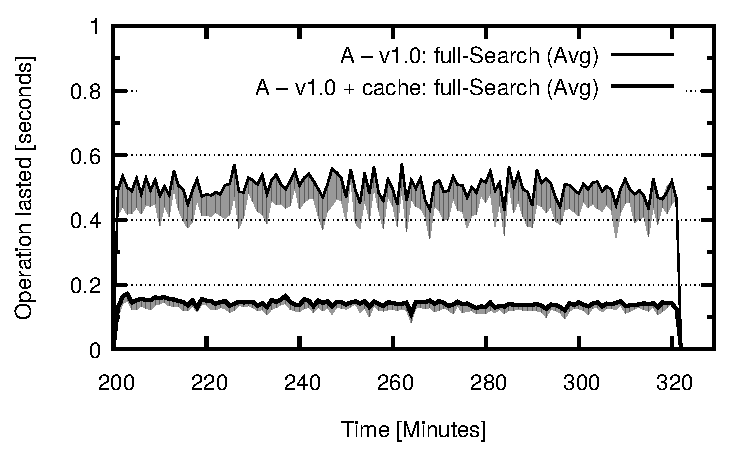
\includegraphics[width=0.98\linewidth]{graphics/fig/Search_Duration_A_10c_fs}
  }
  \\[-1ex]
  \subfigure[A: v1.2 -- Search durations, full-search\label{fig:search_duration_nochurn_12c_fs}] {\centering
  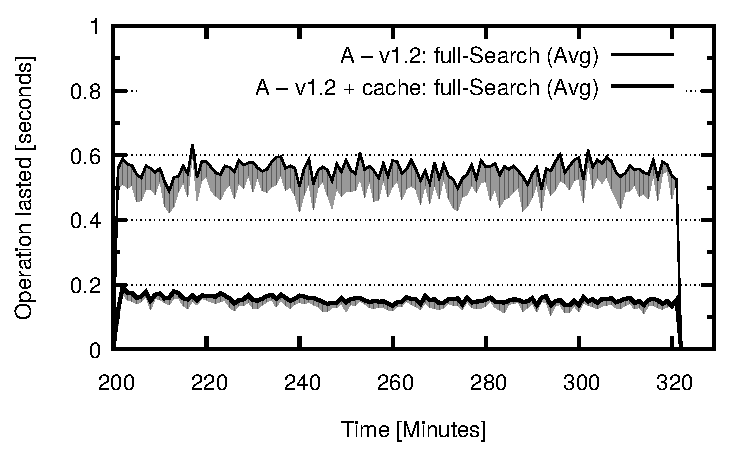
\includegraphics[width=0.98\linewidth]{graphics/fig/Search_Duration_A_12c_fs}
  }
  \\[-1ex]
  \subfigure[A: v1.0 -- Search durations, k-search\label{fig:search_duration_nochurn_10c_ks}] {\centering
  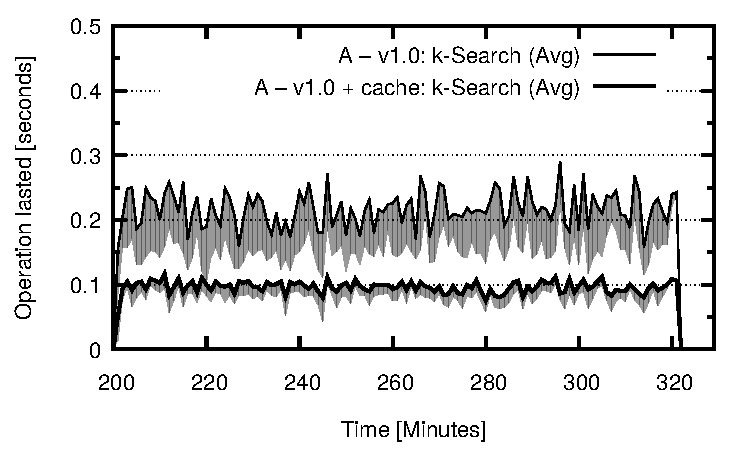
\includegraphics[width=0.98\linewidth]{graphics/fig/Search_Duration_A_10c_ks}
  }
  \\[-1ex]
  \subfigure[A: v1.2 -- Search durations, k-search\label{fig:search_duration_nochurn_12c_ks}] {\centering
  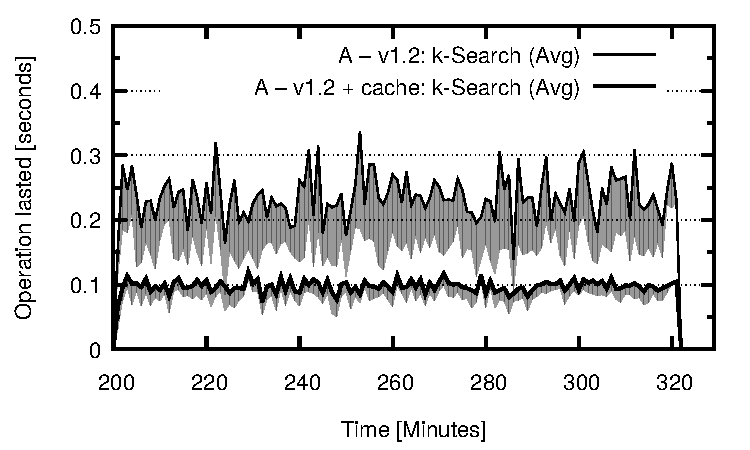
\includegraphics[width=0.98\linewidth]{graphics/fig/Search_Duration_A_12c_ks}
  }
  \\[-1ex]

  \caption{Effetcs of cache and protocol v1.2 on search durations, no churn}
  \label{fig:search_durations_nochurn}
\end{figure}

On the downside, the search duration is slightly affected in v1.2, especially for full searches (compare full-search: Fig.~\ref{fig:search_duration_nochurn_10c_fs} to \ref{fig:search_duration_nochurn_12c_fs}, and k-search: Fig.~\ref{fig:search_duration_nochurn_10c_ks} to \ref{fig:search_duration_nochurn_12c_ks}).
Table~\ref{tab:durations} lists the average search durations for several scenarios.

There is an even more pronounced increase in contacted nodes for a search (search hops), especially for full searches, which is roughly doubling in number (Fig.~\ref{fig:search_hops}).
This is due to the fact that nodes are not allowed to focus their search on the feature with the smallest search range. It is however noteworthy, that our simulations randomized only the lower bound for a search interval. The upper bound is always unlimited. In other words, seekers always search for all occurrences greater or equal a random value. Under this condition a smaller search range is always a best choice. So, we have basically chosen a worst case scenario for the evaluation of the v1.2 protocol revision.

Having said this, the full bandwidth costs for PacketSkip messages (maintenance and search combined) compared to the top 4 overlay message types are clearly enhanced with protocol v1.2 (compare Fig.~\ref{fig:net_C_10} to \ref{fig:net_C_12}).

\begin{figure}[t!]
  \centering
  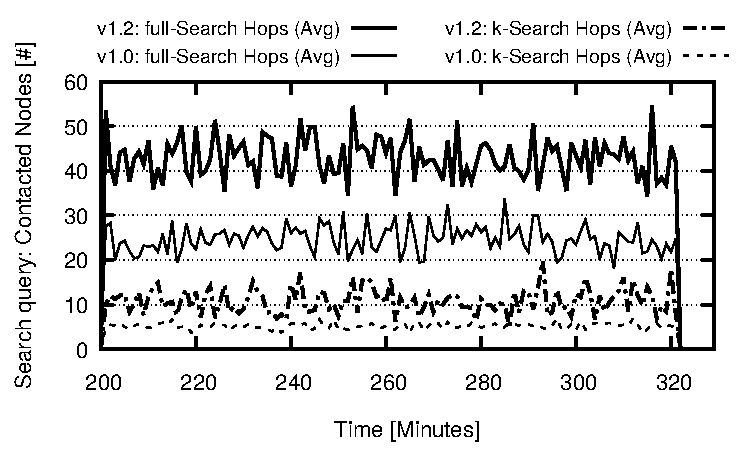
\includegraphics[width=0.98\linewidth]{graphics/fig/Search_Hops}
  \\[-1ex]
  \caption{Effects of protocol revision v1.2 on search hops (full and k-search)}
  \label{fig:search_hops}
\end{figure}


\begin{table}[hb]
\centering
\caption{Average search and update duration times [seconds]}
\label{tab:durations}
\begin{tabular}{|c|c|c|c|c|c|}
\hline
\multirow{2}{*}{\textbf{Scenario}} & \multirow{2}{*}{\textbf{Action}} & \multicolumn{2}{c|}{\textbf{no cache}} & \multicolumn{2}{c|}{\textbf{cache}} \\ \cline{3-6} 
                                   &                                  & \textbf{v1.0}      & \textbf{v1.2}     & \textbf{v1.0}    & \textbf{v1.2}    \\ \hline
                                                                                                                                                        \hline
\multirow{3}{*}{A}                 & Full-Search                      & 0.47               & 0.52              & 0.13             & 0.14             \\ \cline{2-6} 
                                   & k-Search                         & 0.20               & 0.22              & 0.09             & 0.09             \\ \cline{2-6} 
                                   & Update                           & 0.41               & 0.42              & 0.13             & 0.12             \\ \hline
\multirow{3}{*}{B}                 & Full-Search                      & 2.72               & 3.75              & 1.50             & 2.07             \\ \cline{2-6} 
                                   & k-Search                         & 1.11               & 1.18              & 0.64             & 0.84             \\ \cline{2-6} 
                                   & Update                           & 2.06               & 2.05              & 1.31             & 1.19             \\ \hline
\end{tabular}
\end{table}




\subsection{Host cache}
\label{subsec:10c}

We now examine the results of the new host caching component.
As predicted, search and update duration times were considerably reduced in scenario A.
Durations are reduced by a factor of 3.1 on average (Fig.~\ref{fig:search_durations_nochurn}, \ref{fig:update_duration_nochurn_10c}, also table ~\ref{tab:durations}).

A cache may lead to cache misses under churn, so we had to verify its benefits in a more dynamic scenario (B). 
Figures~\ref{fig:search_duration_churn_10_ks} and \ref{fig:search_duration_churn_10c_ks} in comparison demonstrate that our caching mechanism lead to fewer spikes under churn and actually helped to reduce the negative effects of churn on the search duration. 
The update duration is also improved under churn (Fig.~\ref{fig:update_duration_churn_10c}). We measure a reduction of factor 1.7 for searches and updates on average in scenario B (Table~\ref{tab:durations}).


\begin{figure}[htbp]
  \centering

  \subfigure[B: 1.0 -- Search durations without cache under churn\label{fig:search_duration_churn_10_ks}] {\centering
  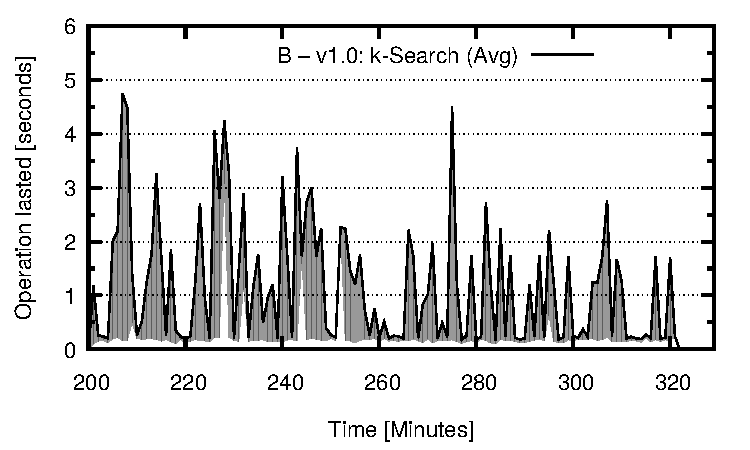
\includegraphics[width=0.98\linewidth]{graphics/fig/Search_Duration_B_10}
  }
  \\[-1ex]
  \subfigure[B: 1.0c -- Search durations with cache under churn \label{fig:search_duration_churn_10c_ks}] {\centering
  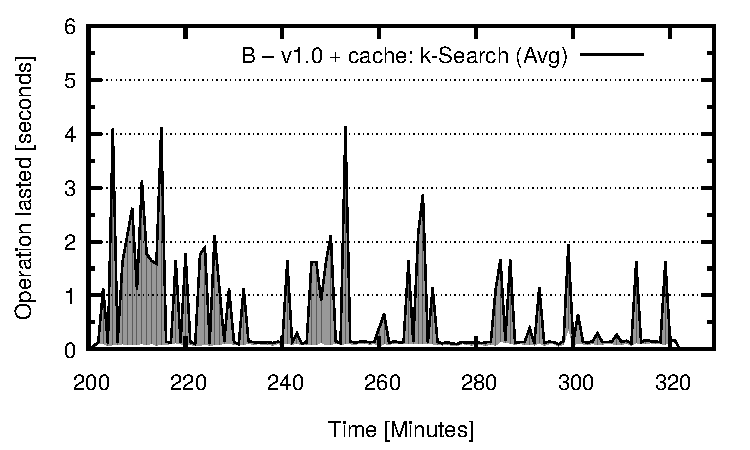
\includegraphics[width=0.98\linewidth]{graphics/fig/Search_Duration_B_10c}
  }
  \\[-1ex]
  \subfigure[A: 1.0 $\rightarrow$ 1.0c -- Update durations, no churn\label{fig:update_duration_nochurn_10c}] {\centering
  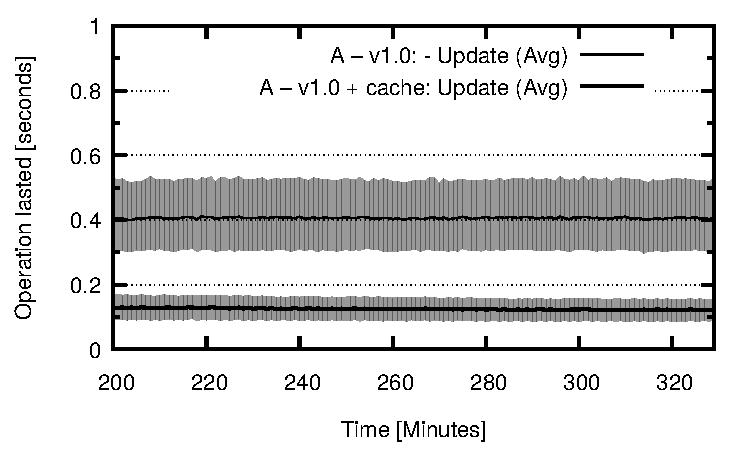
\includegraphics[width=0.98\linewidth]{graphics/fig/Update_Duration_A_10+10c}
  }
  \\[-1ex]
  \subfigure[B: 1.0 $\rightarrow$ 1.0c -- Update durations under churn\label{fig:update_duration_churn_10c}] {\centering
  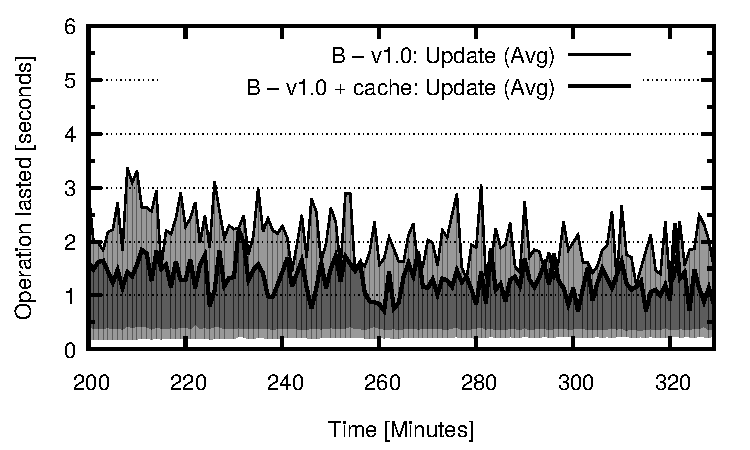
\includegraphics[width=0.98\linewidth]{graphics/fig/Update_Duration_B_10+10c}
  }
  \\[-1ex]

  \caption{V1.0 with cache: influence on search and update durations}
  \label{fig:durations_cache}
\end{figure}






\subsection{Joint enhancements}
\label{subsec:12c}

By avoiding unnecessary lookups we can notably reduce the overlay and lookup traffic caused by PacketSkip. Figure~\ref{fig:net_C_12c} demonstrates the positive effects of all proposed protocol changes in cooperation with the host cache. The entire overlay communication costs are reduced, not only with respect to PacketSkip messages, but especially regarding lookup costs.

As a final note: our evaluation recorded no impact to the accuracy (precision, false positives) of PacketSkip's search results by introducing protocol revisions and host cache.

\begin{figure}[htbp]
  \centering

  \subfigure[C: protocol v1.0\label{fig:net_C_10}] {\centering
  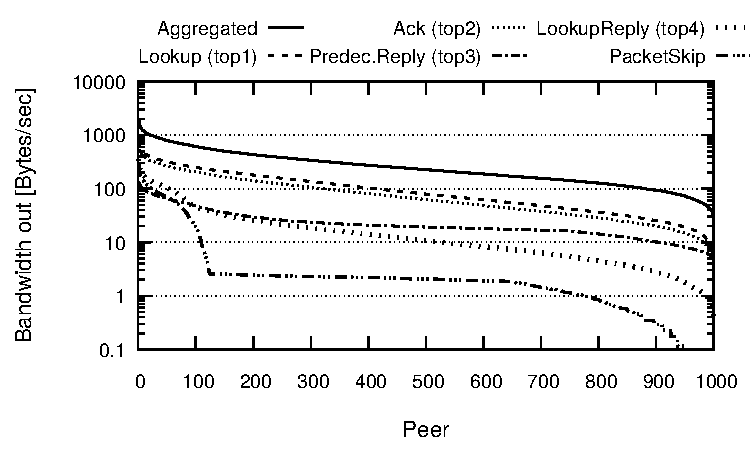
\includegraphics[width=0.98\linewidth]{graphics/fig/Top5_Traffic_Peers_C_10}
  }
  \\[-1ex]

  \subfigure[C: protocol v1.2\label{fig:net_C_12}] {\centering
  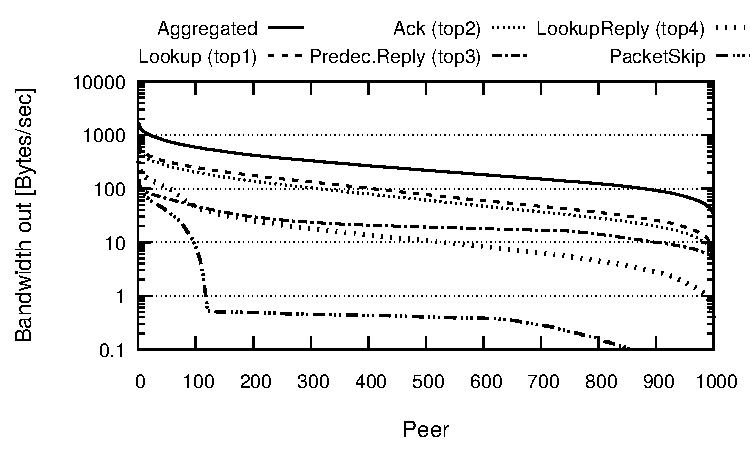
\includegraphics[width=0.98\linewidth]{graphics/fig/Top5_Traffic_Peers_C_12}
  }
  \\[-1ex]
  \subfigure[C: protocol v1.2 + cache\label{fig:net_C_12c}] {\centering
  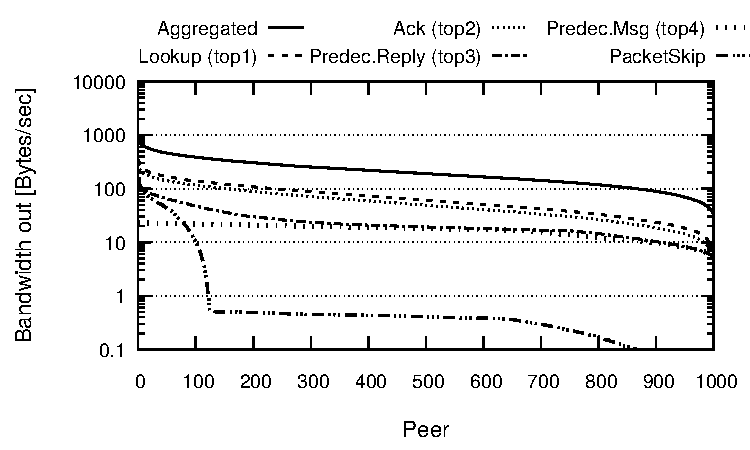
\includegraphics[width=0.98\linewidth]{graphics/fig/Top5_Traffic_Peers_C_12c}
  }
  \\[-1ex]

  \caption{Global overlay traffic: top 4 message types vs PacketSkip}
  \label{fig:net}
\end{figure}


\section{Conclusion / Future Work}
\label{sec:conclusion}

In this paper we have presented two protocol changes for the PacketSkip indexing service. They both address issues of maintenance traffic and storage costs. In combination they reduce average bandwidth demands for update messages by factor 2. Storage costs are reduced by a factor of approximately 1.75, depending on the number of features. The reduction increases with higher dimensionality leading to a better scalability of the service. Search duration is slightly and search hops are more strongly impacted, especially in worst case scenarios.

This is compensated by introducing a communication cache which yields to better update and search performance and reduces the overlay lookup traffic. With all modifications combined we were able to improve the efficiency of the service and boost the capacity retrieval performance significantly without affecting its precision.

For future work it would be interesting to parallelize the service, so that we have multiple PacketSkip graphs at a time. Each of them may be responsible for certain features, either in a 1:1 or 1:$N$ relationship. This should lead to another performance boost and better load balancing of the service on more peers.


\section*{Acknowledgment}

Computational support and infrastructure was provided by the “Center for Information and Media Technology” (ZIM) at the University of D\"usseldorf (Germany).


%\section{Introduction}
%
%\begin{figure}[htb]
%	\centering
%	
\includegraphics[width=0.5\columnwidth]{graphics/hhu}
%	\caption{test figure}
%	\label{fig:test}
%\end{figure}
%
%Motivation of your seminar paper, see Figure \ref{fig:test}. In Section \ref{nextsection} we continue.
%
%
%\section{Next Section}
%\label{nextsection}
%Lorem ipsum dolor sit amet, consetetur sadipscing elitr \cite{chord}, sed diam nonumy eirmod tempor invidunt ut labore et dolore magna aliquyam erat, sed diam voluptua. At vero eos et accusam et justo duo dolores et ea rebum. Stet clita kasd gubergren, no sea takimata sanctus est Lorem ipsum dolor sit amet. Lorem ipsum dolor sit amet, consetetur sadipscing elitr \cite{graffi08icpads}, sed diam nonumy eirmod tempor invidunt ut labore et dolore magna aliquyam erat, sed diam voluptua. At vero eos et accusam et justo duo dolores et ea rebum. Stet clita kasd gubergren, no sea takimata sanctus est Lorem ipsum dolor sit amet.
%
%\begin{itemize}
% \item Lorem ipsum dolor sit amet
% \item consetetur sadipscing elitr
% \item sed diam nonumy eirmod tempor invidunt
% \end{itemize}
%
%\subsection{Subsection}
%Lorem ipsum dolor sit amet, consetetur sadipscing elitr, sed diam nonumy eirmod tempor invidunt (\cite{pastry}) ut labore et dolore magna aliquyam erat, sed diam voluptua. At vero eos et accusam et justo duo dolores et ea rebum. Stet clita kasd gubergren, no sea takimata sanctus est Lorem ipsum dolor sit amet. Lorem ipsum dolor sit amet, consetetur sadipscing elitr, sed diam nonumy eirmod tempor invidunt ut labore et dolore magna aliquyam erat, sed diam voluptua. At vero eos et accusam et justo duo dolores et ea rebum. Stet clita \cite{graffi09lcn} kasd gubergren, no sea takimata sanctus est Lorem ipsum dolor sit amet.
%
%
%\subsection{Subsection with a Table}
%At vero eos et accusam et justo duo dolores et ea rebum, as in \cite{kademlia}. Stet clita kasd gubergren, no sea takimata sanctus est Lorem ipsum dolor sit amet, see Table \ref{table:example}. 
%Lorem ipsum dolor sit amet, consetetur sadipscing elitr, sed diam nonumy eirmod tempor invidunt ut labore et dolore magna aliquyam erat, sed diam voluptua. At vero eos et accusam et justo duo dolores et ea rebum. Stet clita kasd gubergren, no sea takimata sanctus est Lorem ipsum dolor sit amet. Lorem ipsum dolor sit amet, consetetur sadipscing elitr, sed diam nonumy eirmod tempor invidunt ut labore et dolore magna aliquyam erat, sed diam voluptua. At vero eos et accusam et justo duo dolores et ea rebum. Stet clita kasd gubergren, no sea takimata sanctus est Lorem ipsum dolor sit amet.
%
%\begin{table}[htb]
%\centering
%\footnotesize
%\begin{tabular}{|l|l||l|l|}
%\hline
%\textbf{General} & \ & \textbf{Specific}& \ \\
%\hline
%\hline
%A & 1 & 2 & 3 \\
%\hline
%B & 4 & 5 &  6 \\
%\hline
%C & 7 & 8 &  9 \\
%\hline
%\end{tabular}
%\caption{Example table}
%\label{table:example}
%\end{table}


\bibliographystyle{IEEEtran2}
\bibliography{HHU_2017SS_Opp-P2P-Networks___Andreas-Funke___PacketSkip}
\end{document}